\newpage
\chapter{Desenvolvimento}
\label{ch:desenvolvimento}

\par Este capítulo aborda cada uma das etapas do processo de desenvolvimento dos recursos assistivos e implementação da biblioteca ICan.js\footnote{Disponível em: \url{https://icanjs.netlify.com/}}. Os processos detalhados neste capítulo estão na Figura \ref{figure:fluxmethod} representados de maneira geral.

\image{0.18}{imagens_arquitetura/fluxo_de_desenvolvimento_icanjs.png}{Fluxo de desenvolvimento do projeto}{figure:fluxmethod}{Produção do autor}

\par Na Figura \ref{figure:fluxmethod}, inicialmente fez-se a aquisição das imagens de Libras (a), em seguida foi feito o processamento das imagens, treino e distribuição do modelo (b), após isto, a definição do método de conversão da movimentação do usuário para páginas \textit{web} (c) foi definida, por fim, definiu-se a arquitetura da biblioteca e realizou-se a implementação dos recursos assistivos (d).

\section{Arquitetura da biblioteca}

\par A arquitetura da biblioteca, como apresentado anteriormente, foi desenvolvida após as etapas de processamento e criação dos modelos, porém, para a boa compreensão do desenvolvimento deste trabalho, inicialmente é feito a apresentação da biblioteca e sua arquitetura, o que possibilita a fácil ligação de cada um de seus módulos e funções com as citadas na Figura \ref{figure:fluxmethod}.

\par A arquitetura do ICan.js, foi criada seguindo a estrutura apresentada por \citeonline{tensorflowjs2019}, desta forma, a arquitetura é separada em conjuntos de funcionalidades, o que permite um desenvolvimento organizado e uma utilização facilitada. Neste caso, os conjuntos são nomeados \texttt{Core} e \texttt{Common}, que são construídos sobre as funcionalidades disponibilizadas pelo TensorFlow.js e P5.js respectivamente, como apresentado na Figura \ref{figure:icanjsarch}.

\image{0.30}{imagens_arquitetura/arquitetura_camadas_icanjs_v2.png}{Arquitetura do ICan.js}{figure:icanjsarch}{Produção do autor}

\par O conjunto \texttt{Core} é responsável por disponibilizar funcionalidades base para o desenvolvimento dos recursos assistivos, como o acesso a \textit{webcam} dos usuários, os modelos de regressão e também os modelos de rede neural, podendo estes serem carregados de uma \textit{API Rest} de distribuição, ou mesmo do próprio TFJS. Esta camada foi implementada utilizando a especificação ECMAScript 6, o que permitiu o desenvolvimento orientado a objetos mais organizado. As classes desta camada são apresentadas na Figura \ref{figure:icanjscoredc}, onde é evidenciado que, as classes \texttt{PoseNet}, \texttt{CalibrationAPI} e \texttt{MobileNetV1Libras} estendem \texttt{EventEmmiter} do pacote \texttt{events}, isto para que, a interação com estas classes possa ser feita através de eventos, possibilitando a execução assíncrona das classes.

\image{0.16}{imagens_arquitetura/diagrama_de_classe_core.png}{Diagrama de classes da camada \texttt{Core}}{figure:icanjscoredc}{Produção do autor}

\par Por outro lado, há a camada \texttt{Common}, que disponibiliza os recursos assistivos através de funções, criadas com a utilização das funcionalidades da camada \texttt{Core} e também da biblioteca P5.js. Na Figura \ref{figure:icanjsrelacoes} as relações das camadas e bibliotecas utilizadas no ICan.js podem ser vistas.

\image{0.20}{imagens_arquitetura/arquitetura_expandida_icanjs.png}{Relação entre cada uma das camadas}{figure:icanjsrelacoes}{Produção do autor}

\par Para a exposição de cada um dos componentes da Figura \ref{figure:icanjsrelacoes}, as seções seguintes apresentam as etapas do desenvolvimento de cada um dos RAs e seus componentes.

\section{Tradução de Libras para Texto}

\par Este RA permite a interação dos usuários com deficiência auditiva a páginas \textit{web} através de gestos de Libras. As etapas descritas nas subseções abaixo representam os passos a, b e d da Figura \ref{figure:fluxmethod}.

\subsection{Aquisição dos dados}

\par O grande desafio para o desenvolvimento desse RA foi a base de dados, já que, atualmente não há uma base de dados de Libras disponível publicamente \cite{Magalh2018}, de modo a ser necessário a criação para o presente trabalho.

\par A seleção dos gestos que fazem a composição da base de dados foi feita seguindo um critério de identificação, neste é necessário que o gesto possa ser identificado com apenas um \textit{frame}, ou seja, apenas uma imagem é o suficiente para a identificação do gesto, o que torna a RNA aplicada mais simples quando comparada a uma que leva em consideração múltiplas imagens. Desta forma os gestos selecionados foram identificados com essa característica por \citeonline{Magalh2018}, sendo eles (a) Amigo, (b) Desculpa, (c) Telefone, estes apresentados na Figura \ref{figure:gestos_selecionados}.

\begin{figure}[H]
    \centering
    \caption{Gestos selecionados para o conjunto de dados}
    \subfloat[Amigo]{{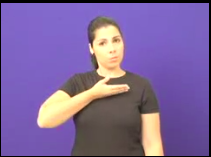
\includegraphics[height=3cm, width=5cm]{src/images/amigo.png}}}%
    \qquad
    \subfloat[Desculpa]{{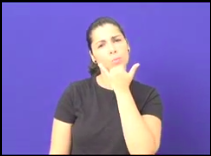
\includegraphics[height=3cm, width=5cm]{src/images/desculpa.png} }}%
    \qquad
    \subfloat[Telefone]{{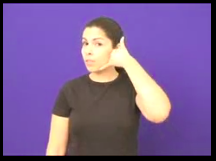
\includegraphics[height=3cm, width=5cm]{src/images/telefone.png} }}%
    \qquad
    \label{figure:gestos_selecionados}%
    \fonte{Adaptado de \citeonline{dicioLibras2011}}
    % \fonte{Produção do autor} % Adaptado de Dicionário de Libras
\end{figure}

\par Para a aquisição dos dados, foi desenvolvido uma ferramenta \textit{desktop} multiplataforma na linguagem Python, com a utilização das bibliotecas PyQt e OpenCV. O fluxo de funcionamento da ferramente é apresentado na Figura \ref{figure:sistema_aquisicao_fluxo}, onde o sistema ao ser iniciado, exibe informações gerais sobre o projeto para o usuário e então já começa o processo de coleta de dados, neste, exemplos dos gestos a serem reproduzidos pelo usuário são exibidos, juntamente a imagem do próprio usuário, além de uma barra de porcentagem para indicar ao usuário seu processo geral na aquisição das imagens.

\image{0.70}{ferramenta_coleta_de_dados/ferramenta_de_aquisicao_fluxo.png}{Tela inicial da aplicação de aquisição de dados}{figure:sistema_aquisicao_fluxo}{Produção do Autor}

\par No total, o sistema captura 60 imagens, sendo 20 para cada um dos gestos. Em cada imagem capturada é aplicado uma operação de redimensionamento para que todas as imagens ao final do processo tenham a dimensão 224x224x3, exigida pela RNC utilizada. Após a aquisição o programa compacta as imagens e às envia por \textit{e-mail}.

\par O programa foi distribuído e ao final houveram 12 colaboradores, criando um conjunto com 720 imagens. Este conjunto de dados foi separado em duas partes, a primeira, com imagens de 11 colaboradores, para o treino e teste do modelo de rede neural, e a segunda, com o colaborador restante, para a validação do modelo. Isso para que, um processo de validação com dados nunca apresentados para a RNC fosse realizado, como forma de assegurar a generalização do modelo, uma vez que, nos dados de treino e teste, mesmo sendo separados nesses dois tipos, possuem imagens dos mesmos participantes.

\subsection{Pré-processamento dos dados}

\par Durante a aquisição das imagens, nenhuma restrição foi imposta aos colaboradores, para tornar o identificador de imagens o mais geral possível, assim, uma etapa de validação de cada uma das imagens teve de ser realizada para garantir que, cada imagem representa o gesto ao qual está vinculada, o que resultou na remoção de algumas imagens. Este processo foi realizado nos dois grupos de dados criados. A Figura \ref{figure:plot_qtd_apos_filtro_por_grupo} apresenta a relação da quantidade de imagens com cada um dos gestos após a verificação dos dados.

\image{1.0}{imagens_pre_processamento_de_dados/plot_grupos_dados_pre_processamento.jpeg}{Quantidade de imagens por gesto após verificação em cada grupo}{figure:plot_qtd_apos_filtro_por_grupo}{Produção do Autor}

\par Após a filtragem, o grupo de dados para treino e teste foi dividido, ficando 80\% dos dados para treino e o restante para teste. Este processo foi criado utilizando a biblioteca sklearn, e o código é apresentado na Figura \ref{figure:split_train_test_data}.

\begin{figure}[H]
    \centering
    \caption{Script de separação dos dados (Treino X Teste)}
    \begin{lstlisting}[language=Python]
from sklearn.model_selection import train_test_split

x, y = [], []

for collaborator_dir in os.listdir():
    files = os.listdir(collaborator_dir)

    x.extend(files)
    y.extend(np.repeat(collaborator_dir, len(files)))

x_train, x_test, y_train, y_test = train_test_split(x, y, test_size=0.20, random_state=992)    
\end{lstlisting}
    \fonte{Produção do autor}
    \label{figure:split_train_test_data}
\end{figure}

\par Nas linhas 5 a 9, a referência do arquivo de cada um dos colaboradores é colocada dentro de listas, cada uma delas representando respectivamente, o arquivo e a classe a qual o arquivo representa, após isto, na linha 11, as listas são divididas em treino e teste.

\par Com a divisão realizada, cada uma das imagens divididas em treino e teste são movidas para os diretórios de seus respectivos tipos com uma função criada em Python (Figura \ref{figure:move_splitted_data}), esta função recebe uma lista com as referências dos arquivos e suas respectivas classes e então copia os arquivos para os devidos diretórios.

\begin{figure}[H]
    \centering
    \caption{Função para movimentação dos arquivos de Treino e Teste}
    \begin{lstlisting}[language=Python]
def move_data(x_data: list, y_data: list, typeof: str) -> None:
    for xt, yt in zip(x_data, y_data):
        src = os.path.join(yt, xt)
        dst = os.path.join(typeof, yt, xt)
        
        copyfile(src, dst)
\end{lstlisting}
    \fonte{Produção do autor}
    \label{figure:move_splitted_data}
\end{figure}

\par Com a finalização da separação dos dados, as quantidades de imagens nos conjuntos de treino/teste podem ser vistas na Figura \ref{figure:qtd_imagem_treino_teste}.

\image{0.35}{imagens_pre_processamento_de_dados/plot_treino_teste.png}{Quantidade de imagens de treino e teste}{figure:qtd_imagem_treino_teste}{Produção do Autor}

\par Poucas imagens podem ser um problema para a generalização do modelo, mesmo levando em consideração a transferência de aprendizado do MobileNet que será feita, assim é aplicado no conjunto de treino, separado anteriormente o \textit{Data Augmentation}. A utilização desta técnica foi feita através da biblioteca Augmentor, onde em um processo iterativo, que passa por todas as imagens do conjunto aplicando certas alterações, e cada uma destas alterações possuem uma probabilidade de ocorrência. A Figura \ref{figure:pipeline_data_augmentation} apresenta o fluxo de processamento do Augmentor e todas as alterações que foram configuradas neste trabalho.

\image{0.60}{imagens_pre_processamento_de_dados/processo_data_augmentation.png}{Fluxo de alterações do processo de \textit{Data Augmentation}}{figure:pipeline_data_augmentation}{Produção do Autor}

\par A implementação do fluxo da Figura \ref{figure:pipeline_data_augmentation} é feita no trecho de código na Figura \ref{figure:dataaugmentation}, nesta, na linha 3 cria-se a instância de um processo de alterações, referenciando o diretório onde estão as imagens que são modificadas para a geração das novas imagens. Da linha 5 a 8 são feitas definições de algumas modificações a serem aplicadas nas imagens, e por fim, na linha 10, 700 imagens são geradas através deste processo.

\begin{figure}[H]
    \centering
    \caption{Trecho do \textit{Script} de \textit{Data Augmentation}}
    \begin{lstlisting}[language=Python]
import Augmentor

p = Augmentor.Pipeline('gestos_editados/treino')

p.random_distortion(probability=0.5, grid_height=3, grid_width=3, magnitude=2)

p.skew_left_right(probability=0.3, magnitude=0.7)
p.skew_corner(probability=0.4, magnitude=0.5)

p.sample(700)
    \end{lstlisting}
    \fonte{Produção do autor}
    \label{figure:dataaugmentation}
\end{figure}

\par A Figura \ref{figure:gestos_gerados_no_pipeline} mostra exemplos de imagens geradas com as diferentes modificações indicadas no código.

\begin{figure}[H]%
    \centering
    \caption{Exemplos de imagens geradas pelo processo de modificação}
    % \subfloat[]{{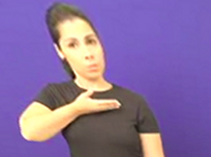
\includegraphics[height=3cm, width=5cm]{src/images/imagens_alteradas_pelo_pipeline/amigo_1.png}}}%
    % \qquad
    \subfloat[]{{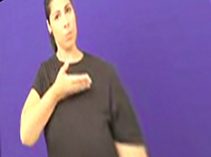
\includegraphics[height=3cm, width=5cm]{src/images/imagens_alteradas_pelo_pipeline/amigo_2.png}}}%
    \qquad
    % \subfloat[]{{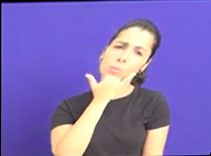
\includegraphics[height=3cm, width=5cm]{src/images/imagens_alteradas_pelo_pipeline/desculpa_1.png}}} %
    % \qquad
    \subfloat[]{{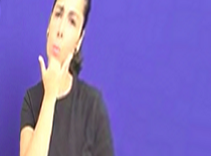
\includegraphics[height=3cm, width=5cm]{src/images/imagens_alteradas_pelo_pipeline/desculpa_2.png}}} %
    \qquad
    \subfloat[]{{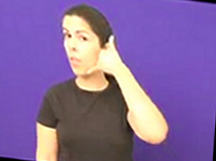
\includegraphics[height=3cm, width=5cm]{src/images/imagens_alteradas_pelo_pipeline/telefone_1.png}}} %
    \qquad
    % \subfloat[]{{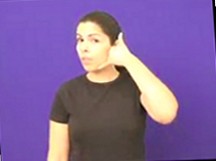
\includegraphics[height=3cm, width=5cm]{src/images/imagens_alteradas_pelo_pipeline/telefone_2.png}}}%
    % \qquad%
    \label{figure:gestos_gerados_no_pipeline}
    \fonte{Produção do autor}
\end{figure}

\par Após a aplicação do \textit{Data Augmentation}, as 700 imagens geradas foram utilizadas como o conjunto de imagens de treino, isto porque, mesmo não havendo uma padrão no momento da aquisição da imagem, muitas delas acabaram ficando semelhantes, por conta da forma de aquisição. A Figura \ref{figure:plot_qtd_apos_dataaugmentation} mostra este valor distribuído por gesto. Com isto, o conjunto de imagens está pronto para ser utilizado no processo de treinamento e teste do modelo de RNC.

\image{0.40}{imagens_pre_processamento_de_dados/plot_qtd_apos_data_augmentation.png}{Quantidade de imagens por gesto com \textit{Data Augmentation}}{figure:plot_qtd_apos_dataaugmentation}{Produção do Autor}

\subsection{Treinamento da Rede Neural Convolucional}

\par O modelo de RNC utilizado neste RA foi o MobileNet, carregado da biblioteca Keras já treinado no conjunto de dados ImageNet \cite{Russakovsky2015}. O modelo carregado foi empregado no desenvolvimento da RA através da técnica de transferência de aprendizado.

\par Esse processo começa com a criação da instância de MobileNet já treinada. Nessa instância não existem a camada de classificação, esta especifica para cada problema, não sendo reutilizável, assim essa camada é adicionada ao modelo instanciado. Na Figura \ref{figure:criacao_do_modelo} o trecho de código para essa criação é apresentado, nesse, na linha 2 é criada a instância do MobileNet, nas linhas 5 e 6 se cria a camada de saída, com um filtro, por fim, nas linhas 9 e 12, são criados o classificador e o novo modelo configurado.

\begin{figure}[H]
    \centering
    \caption{Trecho de código para a criação do modelo}
    \begin{lstlisting}[language=Python]
# Criando o modelo que será retreinado
mobile_net = MobileNet(input_shape=(224, 224, 3), weights='imagenet', include_top=False)

# Configurando o novo topo da rede neural
model_top = mobile_net.output
model_top = GlobalAveragePooling2D()(model_top)

# Classificador
model_top_classifier = Dense(3, activation='softmax')(model_top)

# Gerando novo modelo
new_mobile_net = Model(inputs=mobile_net.input, outputs=model_top_classifier)
    \end{lstlisting}
    \fonte{Produção do autor}
    \label{figure:criacao_do_modelo}
\end{figure}

\par Como citado, neste RA aplicou-se a técnica de transferência de aprendizado no MobileNet, assim foram selecionados para o treinamento todas as camadas após o segundo bloco de convolução, aproveitando as especifidades dos blocos até o segundo e buscando novas características nas camadas a frente. Desta maneira, na Figura \ref{figure:descongelamento_modelo} está o trecho de código para criação do modelo. Na linha 1 todos os blocos de convolução após o segundo são postos para treinamento.

\begin{figure}[H]
    \centering
    \caption{Trecho de código da seleção dos blocos a serem treinados}
    \begin{lstlisting}[language=Python]
new_mobile_net = unfreeze_layers_from(new_mobile_net, 20)
    \end{lstlisting}
    \fonte{Produção do autor}
    \label{figure:descongelamento_modelo}
\end{figure}

\par Com a definição da camada de classificação e das camadas que serão retreinadas, o modelo é configurado com as métricas, funções de otimização e perda utilizadas durante o treinamento. A configuração é feita com o código da Figura \ref{figure:configuracao_do_modelo_para_treino}.

\begin{figure}[H]
    \centering
    \caption{Trecho de código da seleção dos blocos a serem treinados}
    \begin{lstlisting}[language=Python]
new_mobile_net.compile(optimizer=Adam(lr=1e-3), \
        loss='categorical_crossentropy', metrics=['accuracy'])
    \end{lstlisting}
    \fonte{Produção do autor}
    \label{figure:configuracao_do_modelo_para_treino}
\end{figure}

\par Após as configurações, o treinamento do modelo foi realizado com 5 épocas, onde cada uma das épocas representa a quantidade de vezes em que todas imagens do conjunto de dados foi apresentada para a RNC. Todo o processo de treinamento foi realizado utilizando a plataforma Colab com o uso de GPUs, melhorando o resultado e diminuindo o tempo de processamento. A Figura \ref{figure:treinamento_do_modelo} mostra o trecho de código da inicialização do treinamento.

\begin{figure}[H]
    \centering
    \caption{Trecho de código do treinamento do modelo}
    \begin{lstlisting}[language=Python]
new_mobile_net.fit_generator(train_generator,
                            steps_per_epoch=8,
                            epochs=5,
                            validation_data=test_generator,
                            validation_steps=2)

new_mobile_net.save('results/icanv2.h5')
    \end{lstlisting}
    \fonte{Produção do autor}
    \label{figure:treinamento_do_modelo}
\end{figure}

\par No trecho de código da Figura \ref{figure:treinamento_do_modelo}, na linha 7, é evidenciado que o modelo será salvo no formato H5, porém a utilização desse modelo no TFJS requer uma conversão para um formato JSON. Esta conversão é feita na Figura \ref{figure:conversao_do_modelo} e utiliza a ferramenta \texttt{tensorflowjs\_converter}.

\begin{figure}[H]
    \centering
    \caption{Conversão de formato do modelo treinado}
    \begin{lstlisting}[language=sh]
tensorflowjs_converter --input_format keras results/icanv2.h5 \
                                    results_tfjs/
    \end{lstlisting}
    \fonte{Produção do autor}
    \label{figure:conversao_do_modelo}
\end{figure}

\par A utilização da ferramenta (Figura \ref{figure:conversao_do_modelo}) recebe o modelo salvo no formato H5 e o diretório onde o modelo no formato JSON será salvo.

\subsection{Distribuição do modelo}

\par Com a finalização do treinamento e conversão do modelo, foi necessário criar uma forma que facilitasse sua distribuição, uma vez que, para a utilização o TFJS carrega o modelo e todos os seus pesos. Neste caso foi optado pela criação de uma \textit{API Rest}\footnote{Disponível em: \url{https://ican-api.herokuapp.com/}} para a distribuição do modelo, o que evita aos usuários do ICan.js qualquer necessidade de criar suas próprias formas de distribuição do modelo.

\par A \textit{API Rest} foi criada utilizando Python junto ao Flask. A Figura \ref{figure:exemplo_rota_flask} apresenta o código da rota criada para a distribuição do modelo de reconhecimento de Libras.

\begin{figure}[H]
    \centering
    \caption{Rota de distribuição do modelo de reconhecimento de Libras}
    \begin{lstlisting}[language=Python, escapeinside={(*}{*)}]
(*@*)app.route("/models/mobilenetv1/<file>", methods=["GET"])

(*@*)cross_origin()
def mobilenetv1_model(file):
    path = os.path.join(app.config["BASE_DIR"], \
                        "api/models/mobilenetv1")

    try:
        return send_from_directory(directory=path, filename=file)
    except:
        return jsonify({
            "error": True,
            "message": "Erro ao tentar recuperar os dados"
        })
    \end{lstlisting}
    \fonte{Produção do autor}
    \label{figure:exemplo_rota_flask}
\end{figure}

\par Para consumir esta \textit{API} e carregar o modelo na biblioteca, criou-se a classe \texttt{MobileNetV1Libras}, que está no conjunto \texttt{Core} de funcionalidades do ICan.js. O código de consumo da \textit{API} é mostrado na Figura \ref{figure:exemplo_consome_api}.

\begin{figure}[H]
    \centering
    \caption{Método de consumo da \textit{API REST} com o modelo de reconhecimento de Libras}
    \begin{lstlisting}[language=Javascript]
async buildNet() {
    if (this.model === null) {
        this.model = await tf.loadModel(new URL("/models/mobilenetv1/model.json", MODEL_URL).href);
    }
}
    \end{lstlisting}
    \fonte{Produção do autor}
    \label{figure:exemplo_consome_api}
\end{figure}

\par Para que o uso da biblioteca seja rápido, este modelo é carregado uma vez em cada instância de \texttt{MobileNetV1Libras}, desta forma, na linha 2 da Figura \ref{figure:exemplo_consome_api} é verificado se o modelo já foi carregado, caso não tenha sido carregado, a linha 3 é executada e através do TFJS o modelo é carregado em memória.

\subsection{Criação do recurso assistivo}

\par Após todo o processo de coleta de dados, treinamento, disponibilização e consumo do modelo da RNC utilizada neste RA, foi adicionado na camada \texttt{Common} a função \texttt{librasWriter}, que permite a escrita em campos de páginas \textit{web} utilizando gestos de Libras.

\par Como mostrado anteriormente, as imagens utilizadas durante o treinamento do modelo são estáticas, o que faz o \texttt{librasWriter} transcrever a classificação de uma única imagem para texto, porém para garantir a usabilidade, a função também realiza a classificação contínua, isto através do método descrito por \citeonline{Magalh2018}, onde a média dos resultados de classificação feitas em cada uma das imagens capturadas em um intervalo de tempo é utilizado para definir qual foi o gesto realizado pelo usuário. Desta forma, mesmo que o modelo MobileNet retreinado neste trabalho utilize apenas imagens estáticas, pode-se ter uma identificação contínua dos gestos feitos pelo usuário.

\par Essa implementação foi feita no ICan.js permitindo ao usuário inserir o intervalo de tempo (em segundos) que deve ser considerado e também a quantidade de imagens capturadas. O processo de funcionamento da implementação é detalhado na Figura \ref{figure:processo_classificacao_no_tempo}.

\image{0.6}{recurso_assistivo_escrita_com_gestos/processo_de_classificacao_por_media.png}{Processo de classificação de um conjunto de \textit{frames}}{figure:processo_classificacao_no_tempo}{Produção do Autor}

\par Para a implementação do processo da Figura \ref{figure:processo_classificacao_no_tempo} no ICan.js, foi adicionado uma função recursiva (Figura \ref{figure:funcao_recursiva_de_classificacao}) dentro do \texttt{librasWriter}, onde, a linha 3 realiza o processo de classificação de uma imagem, na linha 5 ocorre a verificação da quantidade de imagens já capturadas, e caso a quantidade seja maior ou igual ao definido pelo usuário, a média das classificações é calculada para definir o sinal que em média mais apareceu nas imagens capturadas e então o resultado é enviado para o usuário em um \textit{callback}. Nas linhas 10 a 12 é executado o processo de espera para que, um novo intervalo de tempo seja iniciado.

\begin{figure}[H]
    \centering
    \caption{Função de classificação recursiva}
    \begin{lstlisting}[language=JavaScript]
async function recursiveInterval() {
    try {
        gestures.push(await mobilenetGestures.predictFrame());

        if (gestures.length >= nFrames) {
            fnc(getMeanGesture(gestures));
            gestures = [];
        }

        timeout = window.setTimeout(() => {
            recursiveInterval();
        }, delay * 1000);       
    } catch(err) {
        if (timeout !== null) {
            window.clearTimeout(timeout);
        }

        console.error("librasWriter", err);
    }
}
    \end{lstlisting}
    \fonte{Produção do autor}
    \label{figure:funcao_recursiva_de_classificacao}
\end{figure}

\par Desta forma, os resultados vindos desta função podem ser inseridos em qualquer campo ou formulário de uma página, dependendo apenas da forma como é utilizada no \textit{site}.

\section{Controle do \textit{cursor} do \textit{mouse} com movimentos da cabeça}

\par Este recurso assistivo permite a interação de usuários com deficiência motora a páginas \textit{web} através da movimentação da cabeça. As etapas descritas nas seções abaixo são apresentadas na Figura \ref{figure:fluxmethod} (c, d).

\subsection{Definição do ponto de referência}

\par Para iniciar a criação deste recurso assistivo, foi necessário antes realizar a definição do que seria utilizado como referência para identificar as ações do usuário e mapeá-las para movimentos no \textit{cursor} do \textit{mouse} nas páginas \textit{web}.

\par Este mapeamento pode ser feita de diferentes formas, com técnicas variadas como as apresentadas em \citeonline{Griffin} e \citeonline{Papoutsaki2016}. No contexto deste trabalho decidiu-se utilizar o nariz, que servindo como um ponto de referência, permite ao usuário apontar para qualquer parte da tela (Figura \ref{figure:possiveis_movimentos_nariz}).

\image{0.16}{recurso_assistivo_controle_do_mouse/possiveis_movimentos_com_o_nariz.png}{Movimentação do usuário com o nariz}{figure:possiveis_movimentos_nariz}{Produção do Autor}

\par Com esta definição realizada faz-se necessário aplicar técnicas para a identificação e utilização deste ponto de referência. 

\subsection{Mapeamento dos movimentos do usuário}

\par O mapeamento dos movimentos do usuário, considerando o nariz, exigiu a criação de um processo separado em duas partes, a primeira parte, responsável por identificar o ponto de referência na imagem do usuário e a segunda parte, que através dos resultados de identificação gera os movimentos do \textit{cursor} do \textit{mouse}. Para isso, na etapa de identificação decidiu-se utilizar o modelo PoseNet, e então, o resultado da identificação é aplicado em regressões lineares e seus resultados utilizados para gerar os movimentos do \textit{cursor}, como resumido na Figura \ref{figure:flow_mapeamento}.

\image{0.13}{recurso_assistivo_controle_do_mouse/flow_de_mapeammento_de_movimentos.png}{Fluxo de funcionamento do mapeamento de movimentos para tela do computador}{figure:flow_mapeamento}{Produção do Autor}

\par A aplicação da primeira parte do fluxo (Figura \ref{figure:flow_mapeamento}) no ICan.js é feita através da classe \texttt{PoseNet} (Figura \ref{figure:icanjsrelacoes}), presente na camada de funcionalidades \texttt{Core} da biblioteca. Esta classe carrega o modelo PoseNet (Figura \ref{figure:funcao_carregamento_posenet}) já implementado no TFJS e disponibiliza resultados fazendo o consumo deste modelo.

\begin{figure}[H]
    \centering
    \caption{Método de carregamento do modelo PoseNet}
    \begin{lstlisting}[language=JavaScript]
async buildNet() {
    if (this.neuralModel === null) {
        this.neuralModel = await posenet.load(this.imageMultiplier);
    }
}
    \end{lstlisting}
    \fonte{Produção do autor}
    \label{figure:funcao_carregamento_posenet}
\end{figure}

\par A forma de carregar o modelo do TFJS (Figura \ref{figure:funcao_carregamento_posenet}) não é muito diferente ao apresentado na Figura \ref{figure:exemplo_consome_api}, que carrega o modelo da \textit{API Rest}, a diferença é que, na linha 3, o módulo \texttt{posenet} do TFJS é utilizado para carregar o modelo.

\par Com a identificação da posição do nariz do usuário sendo feita, foi iniciada a segunda etapa do processo de mapeamento dos movimentos, como citado, utilizando regressões lineares. A forma de aplicação das regressões lineares utilizadas neste trabalho no contexto de mapeamento de movimentos, foram descritas por \citeonline{Papoutsaki2016}, onde para que a regressão pudesse ser aplicada neste contexto dois modelos são criados, um para a estimativa de posições horizontais, que possuem como variáveis dependentes e independentes, respectivamente, as posições \textit{X} do \textit{cursor} e do ponto de referência do usuário, neste caso o nariz. Para o segundo modelo, de posições verticais, a mesma lógica é aplicada, porém as variáveis utilizadas são as posições \textit{Y}, do \textit{cursor} e do nariz do usuário. Esta técnica foi implementada na camada \texttt{Core} através da classe \texttt{Regression} e suas especializações (Figuras \ref{figure:icanjscoredc} e \ref{figure:icanjsrelacoes}), onde cada uma destas classes possuem os modelos horizontais e verticais respectivamente.

\par A geração de cada um dos modelos necessita de um processo de ajuste dos coeficiente de regressão, assim no ICan.js foi implementado uma \textit{API} de calibração, que fornece aos utilizadores da biblioteca facilidades para a geração dos coeficientes.

% de geração dos parâmetros regressores, para isto no ICan.js foi implementado uma \textit{API} de calibração, que fornece aos utilizadores da biblioteca facilidades para a geração dos parâmetros regressões.

\subsubsection{Geração dos coeficientes}

\par A geração dos coeficientes de regressão é parte importante para a utilização dos modelos de regressão linear citados anteriormente, para isto, o ICan.js disponibiliza uma \textit{API} de calibração, como apresentado anteriormente. O funcionamento geral desta \textit{API} é evidenciado na Figura \ref{figure:fluxo_api_de_calibracao} e detalhado em seguida.

\image{0.90}{recurso_assistivo_controle_do_mouse/fluxo_de_calibracao.png}{Fluxo de funcionamento da API de calibração}{figure:fluxo_api_de_calibracao}{Produção do Autor}

\par Para a coleta dos pontos utilizados na geração dos coeficientes, fez-se uma implementação que também segue as recomendações apresentadas por \citeonline{Papoutsaki2016}, nessa uma matriz de pontos que cobre as principais posições da tela, possuindo dimensões 3x3 é exibida na tela do usuário (Figura \ref{figure:tela_de_calibracao_da_regressao}), sendo que, quando o usuário clica em cada um destes pontos é salvo a posição do \textit{cursor} e também do nariz do usuário, capturada pelo PoseNet.

\image{0.25}{recurso_assistivo_controle_do_mouse/tela_computador_calibracao_editada.png}{Tela de Calibração}{figure:tela_de_calibracao_da_regressao}{Produção do Autor}

\par Para a implementação da forma de coleta de pontos, inicialmente criou-se no ICan.js a classe \texttt{CalibrationAPI} na camada \texttt{Core}, que fornece regras das posições dos pontos na tela do usuário, além do controle da quantidade de pontos já registrados. Outro recurso implementando na biblioteca foi a função \texttt{calibrate} da camada \texttt{Common}, que junto a biblioteca P5.js gera os pontos especificados pela \texttt{CalibrationAPI} na tela do usuário, coleta as posições do \textit{cursor} (Figura \ref{figure:funcao_coleta_de_pontos_calibracao}) e também do ponto de referência do usuário, neste caso, do nariz, gerado pelo PoseNet, além de gerar os modelos de regressão linear e seus coeficientes.

\begin{figure}[H]
    \centering
    \caption{Função de coleta de pontos}
    \begin{lstlisting}[language=JavaScript]
sketch.mousePressed = function() {
    if (poses !== null) {
        let noseObj = {
            x: poses.keypoints[0].position.x,
            y: poses.keypoints[0].position.y
        }
        
        let mouseObj = {
            x: sketch.mouseX,
            y: sketch.mouseY
        }
        calibrationAPI.isInEllipse(mouseObj, noseObj);
    }
}
    \end{lstlisting}
    \fonte{Produção do autor}
    \label{figure:funcao_coleta_de_pontos_calibracao}
\end{figure}

\par Na Figura \ref{figure:funcao_coleta_de_pontos_calibracao} das linhas 3 a 11 os dados de \textit{X} e \textit{Y} tanto do \textit{cursor} quando do nariz são postos dentro de objetos que são enviados para uma instância de \texttt{CalibrationAPI} na linha 12.

\par Com a quantidade de pontos armazenados atingindo o exigido pelas regras do \texttt{CalibrationAPI}, um evento é enviado para a função \texttt{calibrate}, assim esta cria uma instância da classe \texttt{LinearRegression}, uma especialização de \texttt{Regression} (Figura \ref{figure:icanjscoredc}), separa os pontos coletados em conjuntos contendo respectivamente as posições \textit{X} e \textit{Y} e os utiliza para, através do método \texttt{trainModel} (Figura \ref{figure:funcao_calibracao_modelo_de_regressao}) da instância de \texttt{LinearRegression}, gerar os coeficientes.

\begin{figure}[H]
    \centering
    \caption{Função de calibração dos modelos}
    \begin{lstlisting}[language=JavaScript]
trainModel(xDataset, yDataset) {
    // Verificações omitidas

    // Realiza as regressões para cada um dos datasets
    this.modelX = this.doRegression(xDataset);
    this.modelY = this.doRegression(yDataset);
}
    \end{lstlisting}
    \fonte{Produção do autor}
    \label{figure:funcao_calibracao_modelo_de_regressao}
\end{figure}

\par O método presente na Figura \ref{figure:funcao_calibracao_modelo_de_regressao}, nas linhas 5 e 6 são executados os métodos de treinamento dos modelos de regressão.

\subsection{Criação do recurso assistivo}

\par Com a finalização da implementação do PoseNet e da forma de calibração e utilização do modelo de regressão, foi adicionado na camada \texttt{Common} a função \texttt{screenScroller}, que representa o RA propriamente dito, nesta através da integração das saídas do modelo PoseNet e um modelo de regressão linear já calibrado para o usuário corrente, faz-se as predições do local para onde o usuário está apontando e com o resultado da predição uma \texttt{div} representando um \textit{cursor} criada dentro da página pelo ICan.js tem sua posição alterada para o local predito, isto é feito através do método da Figura \ref{figure:funcao_predicao}.

\begin{figure}[H]
    \centering
    \caption{Função de predição}
    \begin{lstlisting}[language=JavaScript]
sketch.draw = function() {
    if (poses !== null) {
        let nose = poses.keypoints[0];

        let posObj = regressionModel.inferMousePosition(nose);
        changeDivPosition(pointer, posObj.x, posObj.y);

        // Lógica de scrolling
        if (posObj.y < 0) {
            window.scrollTo(0, window.scrollY + posObj.y * 0.05);
        } else if (posObj.y > window.innerHeight) {
            window.scrollTo(0, window.scrollY + (posObj.y - window.innerHeight) * 0.03);
        }
    }
};
    \end{lstlisting}
    \fonte{Produção do autor}
    \label{figure:funcao_predicao}
\end{figure}

\par Na Figura \ref{figure:funcao_predicao}, a linha 1 indica que este método está sendo utilizado dentro de uma instância de \texttt{P5}, sendo que, o método \texttt{draw} cria um laço infinito, o que faz o método descrito estar sempre sendo executado. Já na linha 3, a posição do nariz é recuperada e então na linha 5 passada para uma instância de \texttt{LinearRegression} para que a predição seja realizada, na linha 6 a \texttt{div} criada para representar um \textit{cursor} na página é movida para a posição predita e então das linhas 9 à 13, há uma verificação para saber se é necessário subir ou descer a página.

\par A predição pode representar certa instabilidade, muitas vezes por conta da calibração, desta forma, o ICan.js através da classe \texttt{LinearRegression}, fornece a possibilidade da aplicação de filtros de média e mediana em um conjunto com \textit{N} predições, onde este \textit{N} é definido pelo usuário, assim ao atingir a quantidade de predições necessárias, aplica-se a média ou a mediana nestas predições e o resultado é devolvido. O funcionamento do fluxo de aplicação destes filtros são apresentados na Figura \ref{figure:fluxo_filtro}.

\image{0.60}{recurso_assistivo_controle_do_mouse/fluxo_filtro.png}{Fluxo de funcionamento dos filtros nos resultados das regressões}{figure:fluxo_filtro}{Produção do Autor}

\par Esta técnica de estabilização das predições permite que a movimentação do \textit{cursor} criado seja mais fluída e assertiva, melhorando a usabilidade.
